% =====================================================================
%  LATTICE — Technical Report (NeurIPS-style, SINGLE-FILE)
%  Paste this whole file into Overleaf's main.tex and press Recompile.
%  No extra .sty or .bib files needed — everything is inlined.
%
%  WHERE TO PUT RESULTS:
%   * Headline numbers: the \newcommand block marked "HEADLINE NUMBERS".
%     Fill each once; they flow into the abstract, text, and summary tables.
%   * Table cells: search for \ph (renders as a gray dash) — every empty slot.
%   * Prose to write: search for TODO.
%  Data figures: upload PDFs next to main.tex (same Overleaf folder), e.g.
%  thrb_lattice_unidock_comparison.pdf, thrb_ws2_energy_hist.pdf,
%  ensemble_scaling.pdf.
% =====================================================================
\documentclass[10pt]{article}

% ---------- packages ----------
\usepackage[letterpaper,text={5.5in,9in},top=1in,left=1.5in]{geometry}
\usepackage{mathptmx}                 % Times (as NeurIPS uses)
\usepackage[T1]{fontenc}
\usepackage[utf8]{inputenc}
\usepackage{microtype}
\usepackage[explicit]{titlesec}
\usepackage{booktabs,array,multirow}
\usepackage{graphicx}
\usepackage{tikz}
\usetikzlibrary{positioning,arrows.meta}
\usepackage{amsmath,amssymb}
\usepackage{algorithm}
\usepackage{algpseudocode}
\usepackage{xcolor}
\usepackage{siunitx}
\usepackage{caption}
\usepackage[numbers,sort&compress]{natbib}
\usepackage[colorlinks=true,allcolors=blue!55!black,breaklinks=true]{hyperref}

% ---------- layout / spacing ----------
\setlength{\parindent}{0pt}
\setlength{\parskip}{0.6\baselineskip plus 0.2\baselineskip minus 0.1\baselineskip}
\frenchspacing
\captionsetup{font=small,labelfont=bf,labelsep=period}
\sisetup{table-number-alignment=center,separate-uncertainty=true,table-format=1.3}

% ---------- section headings (NeurIPS-ish) ----------
\titleformat{\section}{\normalfont\large\bfseries}{\thesection}{0.6em}{#1}
\titleformat{\subsection}{\normalfont\normalsize\bfseries}{\thesubsection}{0.6em}{#1}
\titlespacing*{\section}{0pt}{1.4\baselineskip}{0.5\baselineskip}
\titlespacing*{\subsection}{0pt}{1.0\baselineskip}{0.3\baselineskip}

% ---------- centered title + ruled abstract ----------
\makeatletter
\renewcommand{\@maketitle}{%
  \newpage\null\vskip 0.3em%
  \begin{center}%
    {\LARGE\bfseries \@title \par}\vskip 1.2em%
    {\large \@author \par}%
  \end{center}\vskip 1.0em}
\renewcommand{\maketitle}{\par\@maketitle\par\vskip 0.5em}
\makeatother
\renewenvironment{abstract}{%
  \centerline{\rule{\textwidth}{0.4pt}}\vspace{0.4em}%
  \begin{center}{\bfseries Abstract}\end{center}\vspace{-0.2em}\begin{quote}}{%
  \end{quote}\vspace{0.2em}\centerline{\rule{\textwidth}{0.4pt}}\vspace{0.8em}}

% author separators (defined after amssymb so \And isn't clobbered)
\renewcommand{\And}{\hspace{2em}}
\providecommand{\AND}{}\renewcommand{\AND}{\\[0.6em]}

% figure-or-placeholder: shows the PDF if uploaded, else a framed note
\newcommand{\figureorplaceholder}[2]{%
  \IfFileExists{#1}{\includegraphics[width=#2]{#1}}{%
    \fbox{\parbox[c][3.2cm][c]{#2}{\centering\color{gray!70}\small
      \texttt{\detokenize{#1}}\\[2pt] upload this PDF to render the figure}}}}

% =====================================================================
%  HEADLINE NUMBERS  — fill each once (leave as \ph if unknown)
% =====================================================================
\newcommand{\ph}{{\color{gray!70}\,--\,}}
% ---- LIT-PCBA (3-seed ensemble, mean over 15 targets) — FILLED from eval run
\newcommand{\litAUROC}{0.618}   \newcommand{\litBEDROC}{0.081}
\newcommand{\litEFhalf}{10.66}  \newcommand{\litEFone}{6.38}  \newcommand{\litEFfive}{3.24}
% LIT-PCBA (median over targets)
\newcommand{\litAUROCmed}{0.574}\newcommand{\litBEDROCmed}{0.050}
\newcommand{\litEFhalfmed}{3.39}\newcommand{\litEFonemed}{3.09}\newcommand{\litEFfivemed}{2.58}
% ---- Stage-5 held-out BindingDB val split (mean over 3 seeds, 3200 targets)
\newcommand{\valEFone}{21.74}\newcommand{\valEFfive}{8.04}
\newcommand{\valBEDROC}{0.220}\newcommand{\valTopOne}{0.096}
% ---- In-house THR-beta (all 8,368 compounds successfully scored by LATTICE)
\newcommand{\thrbAUROC}{0.826}  \newcommand{\thrbBEDROC}{0.602}
\newcommand{\thrbEFone}{16.46}  \newcommand{\thrbTopHits}{\ph}
% config used for the reported numbers
\newcommand{\sslMethod}{NT-Xent}
\newcommand{\proteinEncoder}{ESM-2 650M}
\newcommand{\nSeeds}{3}\newcommand{\nViews}{4}\newcommand{\bedrocAlpha}{80.5}
\newcommand{\thrbTotal}{8\,369}\newcommand{\thrbBinders}{357}
% ---- THRβ screen timing (amortized s/mol; LATTICE on full library / MI250X)
\newcommand{\thrbLatticeSPerMol}{0.010}\newcommand{\unidockSPerMol}{1.5}\newcommand{\boltzSPerMol}{34}

% training-config constants used throughout the Method section (single source)
\newcommand{\dAdapter}{512}\newcommand{\dProtein}{1280}
\newcommand{\bbBlocks}{6\text{--}10}     % DDiT blocks whose hiddens are concatenated
\newcommand{\encodeTime}{0.98}
\newcommand{\sslTemp}{0.1}\newcommand{\ebmTemp}{0.1}
\newcommand{\sslBatch}{512}\newcommand{\ebmBatch}{64}
\newcommand{\nDecoys}{600}\newcommand{\miningMult}{3}\newcommand{\skipFrac}{5\%}
\newcommand{\fracOther}{0.40}\newcommand{\fracNon}{0.15}\newcommand{\fracRand}{0.45}

% =====================================================================
\title{LATTICE: Sequence-Conditioned Energy-Based Virtual Screening,\\
       Benchmarked on LIT-PCBA and an In-House THR$\beta$ Campaign}


\begin{document}
\maketitle

\begin{abstract}
We present \textbf{LATTICE} (Latent Affinity Training with Target-Informed
Contrastive Estimation), a structure-free virtual-screening model that scores a
protein--ligand pair by a learned energy $E(z_m | z_p)$ conditioned only on the
target's amino-acid sequence. To encode the ligands the
frozen \textbf{InVirtuoGEN} backbone \citep{kaech2025invirtuogen} is used together with an adapter, that is
self-supervised on top. Targets are
encoded by a frozen \proteinEncoder{} protein language model and finally the energy head is trained in a contrastive setup with online hard-negative mining. The model is evaluated on the
held-out LIT-PCBA benchmark, requiring a 90\%
sequence-identity split against BindingDB, and on an in-house campaign against
thyroid hormone receptor~$\beta$ (THR$\beta$). On the held-out BindingDB
validation split the \nSeeds{} heads reach EF@1\% $=\valEFone$ and BEDROC
$=\valBEDROC$. Transferring to LIT-PCBA, the \nSeeds{}-seed ensemble reaches a
mean EF@1\% of \litEFone{} and BEDROC of \litBEDROC{} (mean AUROC \litAUROC{});
the ensemble outperforms every individual seed on every metric. On the
\thrbTotal{}-compound THR$\beta$ library the same models recover \thrbBinders{}
labelled binders with AUROC \thrbAUROC{} and EF@1\% \thrbEFone{}. % TODO: THR-beta screen not
% yet run — those four numbers are still placeholders.
\end{abstract}

% ---------------------------------------------------------------------
\section{Introduction}
Most accurate virtual-screening methods rely on the target's three-dimensional
structure (a co-crystal pocket, a docking grid, or a predicted fold), which is
not always available, is expensive to prepare per target, and ties throughput to
the cost of posing each ligand. We instead ask what can be achieved from the
target's amino-acid sequence alone: no explicit 3D structure, no defined binding
pocket, and no docking pose. This is a weaker input than structure-based docking,
but a far cheaper and more scalable one, and it lets a single trained model score
any library against any target for which a sequence is known. It is not
``structure-free'' in a strong sense, since the protein language model we use
(\proteinEncoder{}) is trained on evolutionary data and encodes structural and
functional signal implicitly, but it requires no experimental or predicted
structure as input.

This report presents \textsc{lattice}, a sequence-based, target-conditioned
energy-based screener, and present results on the public
LIT-PCBA benchmark \citep{tran2020litpcba} and on an internal THR$\beta$ campaign.
LATTICE builds directly on the prior published model,
\textbf{InVirtuoGEN} \citep{kaech2025invirtuogen}. InVirtuoGEN learns a
discrete flow over fragmented SMILES to \emph{generate} drug-like molecules, here
we repurpose its pretrained backbone as a frozen molecular \emph{encoder} and
learn, on top of it, a sequence-conditioned energy head that \emph{ranks} molecules
against a target. Our contributions are:
\begin{itemize}
  \item A sequence-based virtual-screening model that reuses the frozen
        InVirtuoGEN discrete-flow backbone as a molecule encoder, adds a
        self-supervised adapter, and learns a target-conditioned energy head
        by InfoNCE with hard-negative mining.
  \item A leakage-controlled LIT-PCBA evaluation (90\% identity split vs.\
        BindingDB) reporting AUROC, BEDROC and enrichment factors
        (Section~\ref{sec:litpcba}).
  \item An in-house THR$\beta$ screen of \thrbTotal{} compounds with retrieval
        metrics and a head-to-head comparison against Uni-Dock, Boltz-2, and
        Nesso-1 (Section~\ref{sec:thrb}).
\end{itemize}
% ---------------------------------------------------------------------
\section{Method}\label{sec:method}
\begin{figure}[t]\centering
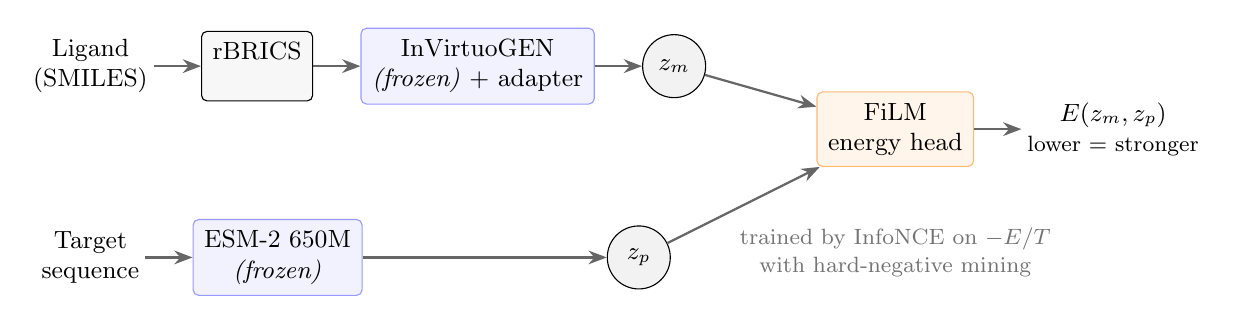
\begin{tikzpicture}[font=\small,>=Stealth,node distance=6mm,
    box/.style={draw,rounded corners=2pt,align=center,inner sep=4pt,minimum height=8mm,fill=black!3},
    frozen/.style={box,fill=blue!5,draw=blue!40},
    head/.style={box,fill=orange!8,draw=orange!55},
    lat/.style={draw,circle,inner sep=1.2pt,fill=black!5,minimum size=8mm},
    io/.style={align=center,inner sep=2pt}, ar/.style={->,thick,draw=black!60}]
  \node[io] (smiles) {Ligand\\(SMILES)};
  \node[box,right=of smiles] (brics) {rBRICS\\};
  \node[frozen,right=of brics] (ddit) {InVirtuoGEN\\\textit{(frozen)} + adapter};
  \node[lat,right=of ddit] (zm) {$z_m$};
  \node[io,below=16mm of smiles] (seq) {Target\\sequence};
  \node[frozen,right=of seq] (esm) {ESM-2 650M\\\textit{(frozen)}};
  \node[lat,right=31mm of esm] (zp) {$z_p$};
  \node[head,right=14mm of zm,yshift=-8mm] (film) {FiLM \\ energy head};
  \node[io,right=of film] (energy) {$E(z_m,z_p)$\\\footnotesize lower $=$ stronger};
  \draw[ar](smiles)--(brics); \draw[ar](brics)--(ddit); \draw[ar](ddit)--(zm);
  \draw[ar](seq)--(esm); \draw[ar](esm)--(zp);
  \draw[ar](zm)--(film); \draw[ar](zp)--(film); \draw[ar](film)--(energy);
  \node[io,below=7mm of film,text=black!55]{\footnotesize trained by InfoNCE on $-E/T$\\[-1pt]
     \footnotesize with hard-negative mining};
\end{tikzpicture}
\caption{The LATTICE scoring pipeline. The molecule and target are encoded
independently by frozen language models (a DDiT SMILES backbone with a
self-supervised adapter, and \proteinEncoder{}); a FiLM (Feature-wise Linear
Modulation) head \citep{perez2017filmvisualreasoninggeneral} conditions the molecule representation on
the target and maps the two latents to a scalar energy $E$, and the library is
ranked by $-E$.}\label{fig:arch}
\end{figure}

LATTICE couples two frozen pretrained encoders with a single trained energy head.
The molecule encoder is first pretrained by self-supervision
(Section~\ref{sec:ssl}); both encoders are then frozen and used to precompute
molecule and protein latents, on top of which only the energy head is trained
(Section~\ref{sec:ebm}). The components are described in turn below.

\subsection{Molecule encoder: InVirtuoGEN-SSL}
InVirtuoGEN operates on fragmented SMILES, where the revised BRICS algorithm \citep{rbrics} is used for the fragmentation. The resulting strings are tokenized with an atom-level vocabulary. InVirtuoGEN's backbone is reused purely as a molecule encoder: the fragment token
sequence is run at a fixed, near-clean encode-time $t=\encodeTime$ on the flow
trajectory, the hidden states of blocks~\bbBlocks{} are concatenated, and a
lightweight \emph{adapter} is trained on top.
The adapter linearly projects the concatenated hiddens to width $\dAdapter$, mixes
them with a $2$-layer bidirectional transformer to produce the molecule latent
$z_m\in\mathbb{R}^{\dAdapter}$ via pooling.

\paragraph{Self-supervised pretraining}\label{sec:ssl}
Before it is trained for screening, the molecule encoder is pretrained on the
$\sim$1.6M drug-like molecules of MOSES \citep{polykovskiy2020moses} with a
contrastive objective (NT-Xent) \citep{chen2020simpleframeworkcontrastivelearning}.
The idea is simple: each molecule is presented to the encoder in two randomly
fragmented versions, and the encoder learns to place those two views close together in
latent space while pushing them away from the views of every other molecule in the
batch. Repeated over many batches, this yields a representation that reflects
chemical identity rather than superficial details of how the molecule was written
down.

Concretely, for a batch of $B$ molecules we form $2B$ views. Writing $z_i$ for the
normalized embedding of view $i$, we minimize the symmetric NT-Xent loss
\begin{equation}
\mathcal{L}_{\text{NT-Xent}}
= \frac{1}{2B}\sum_{i=1}^{2B}
-\log\frac{\exp\!\big(\mathrm{sim}(z_i, z_{p(i)})/T\big)}
{\sum_{k\neq i}\exp\!\big(\mathrm{sim}(z_i, z_k)/T\big)},
\label{eq:ntxent}
\end{equation}
where $\mathrm{sim}$ is cosine similarity, $T=\sslTemp$ is a temperature, and
$p(i)$ indexes the matching view of the same molecule. Every other view in the
batch acts as a negative, so a larger batch simply supplies more negatives per
step.
\paragraph{Fingerprint similarity distillation.}
Alongside the contrastive loss, an auxiliary term encourages the latent geometry
to match classical chemical similarity. For each batch we compute the pairwise
cosine similarities of the L2-normalized molecule embeddings and the pairwise
Tanimoto similarities of their Morgan fingerprints, then regress the former onto
the latter over all non-self pairs. Molecules that share substructure (high
Tanimoto) are pulled closer in embedding space while dissimilar molecules are
pushed apart, with no contrastive positives or negatives and no temperature, just
a direct match of the two similarity matrices. This term is added with a controllable
weight $\lambda_{\text{fp}}$.
\begin{algorithm}[t]
\caption{Contrastive pretraining step (one minibatch of $B$ molecules)}
\label{alg:ntxent}
\begin{algorithmic}[1]
\State \textbf{input:} molecules $\{s_i\}_{i=1}^{B}$, temperature $T$, weight $\lambda$
\For{$i = 1 \ldots B$}
  \State $a_i,\ b_i \gets$ two random fragmentations of $s_i$ \Comment{e.g.\ fragment-order permutations}
\EndFor
\State $z^a \gets \textsc{L2Norm}(\textsc{Encoder}(a))$;\quad $z^b \gets \textsc{L2Norm}(\textsc{Encoder}(b))$
\State $\mathcal{L} \gets \mathcal{L}_{\text{NT-Xent}}(z^a, z^b) + \lambda\,\mathcal{L}_{\text{chem}}$ \Comment{Eq.~\eqref{eq:ntxent}; in-batch negatives + align with chemical similarity}
\State \textbf{update} encoder
\end{algorithmic}
\end{algorithm}

\subsection{Protein encoder: ESM-2}\label{sec:protenc}
The protein sequences are embedded by a frozen pretrained \proteinEncoder{} model
\citep{lin2023esm2}; the latent representations of the last layer are mean-pooled to a single vector
$z_p\in\mathbb{R}^{\dProtein}$.

\subsection{Energy head and training}\label{sec:ebm}
The energy head is the only component trained for screening. It takes a molecule
latent $z_m$ and a target latent $z_p$ and returns a scalar energy $E(z_m, z_p)$,
where a lower energy denotes a stronger predicted binder (Figure~\ref{fig:arch}).
The target conditions the computation through FiLM: $z_p$ is mapped to a set of
per-feature scales and shifts that modulate the molecule features before a small
network reduces them to the final energy. The modulation is initialized so that
the head begins by ignoring the protein condition and gradually learns to use it.

\paragraph{Latent pools.}
Training draws on two sources: MOSES \citep{polykovskiy2020moses}, a library of
drug-like molecules, and BindingDB \citep{gilson2016bindingdb}, a database of
protein--ligand pairs with activity annotations. Targets and their labelled
actives and inactives are taken from BindingDB, while MOSES provides additional
unlabelled molecules used as generic decoys. As both encoders are frozen, latents
are precomputed and cached rather than recomputed at each step: a target pool of
protein latents $z_p$, and molecule pools of confirmed actives, annotated
BindingDB ligands, and generic MOSES decoys.

\paragraph{Hard-negative mining.}
Each minibatch comprises \ebmBatch{} targets, each pairing one binder $z_m^{+}$
with \nDecoys{} decoys assembled from the pools by a fixed mixture
(Table~\ref{tab:decoymix}) and refined by hard-negative mining. Because most decoys
are already scored well below the binder and contribute little gradient, the
candidate set is oversampled and scored with the current head, and only the hardest
are retained. The few lowest-energy candidates are discarded, as a decoy scoring as
high as a binder is likely an unlabelled active.

\begin{algorithm}[t]
\caption{Hard-negative mining (per target)}
\label{alg:hardneg}
\begin{algorithmic}[1]
\State \textbf{input:} binder $z_m^{+}$, target $z_p$; counts $N{=}\nDecoys$, multiplier $m{=}\miningMult$, skip $\rho{=}0.05$
\State draw $N\!\cdot\!m$ candidate decoys $\{z_m^{-}\}$ from the mix in Table~\ref{tab:decoymix}
\State $e^{-} \gets E(z_m^{-}, z_p)$ for all candidates \Comment{current head, no grad}
\State $\pi \gets \textsc{ArgSort}(e^{-})$ \Comment{ascending: hardest (lowest $E$) first}
\State $\text{skip} \gets \lfloor \rho\,N m \rceil$ \Comment{drop likely false negatives}
\State keep $\{z_m^{-}\}_{\pi[\text{skip}\,:\,\text{skip}+N]}$ as the target's decoys
\State $e^{+} \gets E(z_m^{+}, z_p)$;\quad form logits $[-e^{+}/T, -e^{-}_1/T, \ldots, -e^{-}_N/T]$
\State $\mathcal{L}_{\text{InfoNCE}} \gets \textsc{CrossEntropy}(\text{logits},\ \text{target}{=}0)$ \Comment{binder at index 0}
\end{algorithmic}
\end{algorithm}

\begin{table}[t]\centering
  \caption{Composition of the \nDecoys{} decoys drawn per binder in a training
  batch. Fractions are the training defaults; the two BindingDB buckets are the
  ``hard'' negatives, the MOSES bucket provides coverage. Under hard-negative
  mining these counts describe the \emph{candidate} pool, oversampled by
  $\times\miningMult$ before mining (Algorithm~\ref{alg:hardneg}).}
  \label{tab:decoymix}\small\setlength{\tabcolsep}{7pt}
  \begin{tabular}{l l S[table-format=1.2] S[table-format=3.0]}
    \toprule
    Source & Role & {Fraction} & {Count} \\
    \midrule
    BindingDB cross-target binders & drug-like hard negative & 0.40 & 240 \\
    BindingDB annotated non-binders & assay-confirmed inactive & 0.15 & 90 \\
    MOSES random & chemical-space coverage & 0.45 & 270 \\
    \midrule
    \textbf{Total} & & 1.00 & 600 \\
    \bottomrule
  \end{tabular}
\end{table}

\paragraph{Training objective.}
Given a binder and its mined decoys, the head is trained with a contrastive
(InfoNCE) loss that pushes the binder's energy below every decoy's for that target.
Two auxiliary terms support it: a distribution-matching (Sinkhorn) term shapes the
overall spread of binder and decoy energies rather than only their relative order,
and a cross-target term scores each binder against a wrong protein from the batch
and requires it to look worse there than against its true target, an explicit check
that the energy genuinely depends on the sequence. At inference, each molecule's
latent is averaged over \nViews{} fragmentations and \nSeeds{} independently
trained heads are ensembled, then the library is ranked by $-E$.
\section{Experimental setup}\label{sec:setup}
\paragraph{Training data.}
To prevent leakage into LIT-PCBA, BindingDB targets are clustered with MMseqs2 and
split at 90\% sequence identity against the LIT-PCBA targets; only the held-out
partition is used for training.
\paragraph{Benchmarks and metrics.}
LIT-PCBA \citep{tran2020litpcba} provides 15 targets with experimentally
validated actives and property-matched inactives. We report ROC-AUC, BEDROC at
$\alpha{=}\bedrocAlpha$ \citep{truchon2007bedroc}, and enrichment factors EF@0.5\%,
EF@1\% and EF@5\%, averaged (mean and median) across targets. The in-house
THR$\beta$ library (Section~\ref{sec:thrb}) is scored with the same models and
metrics on THR$\beta$ labels.

% ---------------------------------------------------------------------
\section{Results on holdout \& LIT-PCBA}\label{sec:litpcba}
Before turning to LIT-PCBA we report performance on the held-out BindingDB
validation split, which shares its target distribution with training and so
measures in-distribution ranking (Table~\ref{tab:bdbval}). Ranking $\nDecoys$
decoys per target across $3{,}200$ targets, the heads reach EF@1\% $=\valEFone$
and BEDROC $=\valBEDROC$, i.e.\ roughly a $22\times$ enrichment over random in the
top percentile, with the true binder ranked first about $10\%$ of the time.

\begin{table}[h]\centering
  \caption{Held-out BindingDB validation split (Stage-5 protocol: one binder vs.\
  \nDecoys{} decoys per target, $3{,}200$ targets). Mean $\pm$ s.d.\ over the
  \nSeeds{} seeds. This is in-distribution performance; LIT-PCBA
  (Table~\ref{tab:litpcba}) is the out-of-distribution test.}
  \label{tab:bdbval}\small\setlength{\tabcolsep}{7pt}
  \begin{tabular}{l S[table-format=2.2] S[table-format=1.2] S[table-format=1.3] S[table-format=1.3]}
    \toprule
    Seed & {EF@1\%} & {EF@5\%} & {BEDROC} & {Top-1 acc.} \\
    \midrule
    0 & 22.07 & 8.04 & 0.224 & \textbf{0.101} \\
    1 & 20.28 & 7.67 & 0.204 & 0.087 \\
    2 & \textbf{22.88 }&\textbf{ 8.40} & \textbf{0.231} & \textbf{0.101} \\
    \midrule
    \textbf{Mean} & \valEFone & \valEFfive & \valBEDROC & \valTopOne \\
    \bottomrule
  \end{tabular}
\end{table}

On LIT-PCBA (Table~\ref{tab:litpcba}) the \nSeeds{}-seed ensemble reaches mean
AUROC $\litAUROC$, BEDROC $\litBEDROC$ and EF@1\% $=\litEFone$. The ensemble outperforms the individual seeds on almost every considered metric.

Table~\ref{tab:litpcba-baselines} places the ensemble against representative
baselines.

\begin{table}[h]\centering
  \caption{LIT-PCBA performance, aggregated over the 15 targets. Each seed is an
  independently-initialized energy head trained on the same \sslMethod{} adapter;
  ``Ensemble'' averages the \nSeeds{} energies before ranking (\nViews{}-view
  $z_m$, \proteinEncoder{} target embeddings; BEDROC $\alpha=\bedrocAlpha$).}
  \label{tab:litpcba}\small\setlength{\tabcolsep}{6pt}
  \begin{tabular}{l S[table-format=1.3] S[table-format=1.3] S[table-format=2.2] S[table-format=1.2] S[table-format=1.2]}
    \toprule
    Model & {AUROC} & {BEDROC} & {EF@0.5\%} & {EF@1\%} & {EF@5\%} \\
    \midrule
    Seed 0 & 0.617 & 0.075 & 8.59 & 6.20 & 3.09 \\
    Seed 1 & 0.603 & 0.071 & 8.35 & 6.20 & 2.81 \\
    Seed 2 & 0.599 & 0.074 & 8.99 &\textbf{ 6.57 }& 2.93 \\
    \midrule
    \textbf{Ensemble (\nSeeds{})} & \textbf{\litAUROC} & \textbf{\litBEDROC} & \textbf{\litEFhalf} & \litEFone & \textbf{\litEFfive} \\
    \bottomrule
  \end{tabular}
\end{table}
% OPTIONAL per-target breakdown: the eval run above reports only the aggregate.
% To add a per-target table, read artifacts/ablation/evaluation/<run>/lit_pcba_mv4.csv
% (one row per target: auroc, bedroc, ef@0.5%, ef@1%, ef@5%) and paste the 15 rows here.
\begin{table}[h]\centering
  \caption{Mean LIT-PCBA performance versus DrugCLIP and h-MINT. Baseline
  figures are those reported by \citet{gao2023drugclip} and
  \citet{qu2026hmintmodelingpocketligandbinding}; percentage-valued AUROC and BEDROC are shown here as
  fractions. Differences in training data and evaluation protocol make the
  comparison indicative rather than strictly head-to-head.}
  \label{tab:litpcba-baselines}\small\setlength{\tabcolsep}{6pt}
  \begin{tabular}{l l S[table-format=1.4] S[table-format=1.2] S[table-format=1.4]}
    \toprule
    Method & Target repr. & {AUROC} & {EF@1\%} & {BEDROC} \\
    \midrule
    DrugCLIP \citep{gao2023drugclip} & pocket & 0.5717 & 5.51 & 0.0623 \\
    h-MINT \citep{qu2026hmintmodelingpocketligandbinding} & pocket & 0.5777 & 5.20 & 0.0627 \\
    \midrule
    \textbf{LATTICE (ours)} & \proteinEncoder{} seq. & \bfseries\textbf{\litAUROC} &  \bfseries\textbf{\litEFone} & \bfseries\textbf{\litBEDROC} \\
    \bottomrule
  \end{tabular}
\end{table}

\paragraph{How many energy heads to ensemble?}
To choose $\nSeeds{}$, we trained nine independently initialized FiLM heads on the
same \sslMethod{} adapter and measured how mean LIT-PCBA BEDROC and AUROC scale
with the ensemble size $k$ (Figure~\ref{fig:ensemble-scaling}). For each $k$, the library
is ranked by the average of $k$ head energies; over every subset of size $k$ the
mean BEDROC rises from $0.068$ ($k{=}1$) toward $0.078$ ($k{=}9$) while the
subset-to-subset standard deviation shrinks. The sequential curve that always
takes seeds $0{\ldots}k{-}1$ sits above the all-subset mean for $k<9$ and is
already near its maximum at $k{=}3$: adding the fourth head changes BEDROC by
only $0.00013$. We therefore report the \nSeeds{}-seed ensemble as a compact
operating point, rather than selecting the largest ensemble after observing the
test set. The best-subset curve is included only as a post-hoc upper envelope:
because it selects heads using LIT-PCBA labels, it is optimistic and is not a
valid prospective selection procedure.

\begin{figure}[t]\centering
  \figureorplaceholder{ensemble_scaling.pdf}{\linewidth}
  \caption{Energy-averaging ensemble scaling on LIT-PCBA (nine FiLM heads on the
  same adapter). \textbf{a}, BEDROC ($\alpha=\bedrocAlpha$), emphasizing early
  recognition. \textbf{b}, AUROC, measuring global ranking. Solid: mean $\pm$
  s.d.\ over all $\binom{9}{k}$ subsets of size $k$. Dashed: sequential seeds
  $0{\ldots}k{-}1$ in submission order.
  Dotted: the best size-$k$ subset selected post hoc on LIT-PCBA. The shaded band
  measures sensitivity to which heads are selected; it is not a confidence
  interval over targets or training runs. All curves meet at $k{=}9$ because
  only one full-set ensemble exists. Heads share the same cached molecular and
  protein latents; their scalar energies are averaged before ranking.}
  \label{fig:ensemble-scaling}
\end{figure}

% ---------------------------------------------------------------------
\newpage
\section{In-house THR$\beta$ virtual screen}\label{sec:thrb}
We applied the trained models to an internal campaign against thyroid hormone
receptor~$\beta$. The evaluation library (Table~\ref{tab:thrb-dataset}) merges
ChEMBL experimental actives/inactives, the WS1 and Rapposelli medicinal-chemistry
series, and property-matched decoys, for \thrbTotal{} standardized compounds of
which \thrbBinders{} carry a THR$\beta$ binder label.

\begin{table}[h]\centering
  \caption{Composition of the in-house THR$\beta$ evaluation library
  ($8{,}369$ standardized compounds). Labels are THR$\beta$ assay activity only;
  property-matched decoys are presumed inactive.}
  \label{tab:thrb-dataset}\small\setlength{\tabcolsep}{7pt}
  \begin{tabular}{l S[table-format=4.0] S[table-format=3.0] S[table-format=4.0]}
    \toprule
    Source & {Compounds} & {THR$\beta$ binders} & {Non-binders} \\
    \midrule
    ChEMBL experimental     & 713  & 353 & 360  \\
    WS1\_v1                  & 110  & 0   & 110  \\
    WS1\_v2                  & 104  & 1   & 103  \\
    Rapposelli              & 4    & 3   & 1    \\
    Property-matched decoys & 7438 & 0   & 7438 \\
    \midrule
    \textbf{Total}          & 8369 & 357 & 8012 \\
    \bottomrule
  \end{tabular}
\end{table}

\paragraph{Retrieval performance.}
Table~\ref{tab:thrb-metrics} reports early-recognition metrics when ranking the
library by predicted THR$\beta$ affinity. For a direct comparison, metrics are
computed on the compounds jointly scored by LATTICE, Uni-Dock, Boltz-2
\citep{passaro2025boltz2}, and Nesso-1 \citep{valencelabs2026nesso1}: the
ChEMBL set and property-matched decoys ($n{=}8{,}150$). LATTICE reaches
EF@1\% $=16.33$ and BEDROC $=0.607$, ahead of Uni-Dock ($10.42$ / $0.469$) and
well ahead of Boltz-2 ranked by its affinity probability ($3.10$ / $0.106$).
Nesso-1 is a recent open-source coarse-grained cofolding affinity model
\citep{valencelabs2026nesso1}; its THR$\beta$ numbers are pending (Table~\ref{tab:thrb-metrics}).
Figure~\ref{fig:thrb-comparison} compares global discrimination and, more
importantly for prospective screening, enrichment within the first 10\% of the
ranked library. LATTICE provides the largest gain at the most selective cutoffs
(EF@0.5\% and EF@1\%), while LATTICE and Uni-Dock become more similar by 5\%;
Boltz-2 remains near-random on early enrichment throughout.

\begin{table}[H]\centering
  \caption{THR$\beta$ retrieval performance on the 8,150 compounds jointly
  scored by LATTICE, Uni-Dock \citep{yu2023unidock}, Boltz-2
  \citep{passaro2025boltz2}, and Nesso-1 \citep{valencelabs2026nesso1}
  (353 ChEMBL binders and 7,797 ChEMBL inactives/property-matched decoys).
  Lower LATTICE energies and Uni-Dock scores rank first; Boltz-2 uses its
  affinity probability (higher first). BEDROC uses $\alpha=\bedrocAlpha$.
  The s/mol column is amortized wall-clock per molecule (LATTICE: encode+score
  on one MI250X; Uni-Dock: SDF prep+dock; Boltz-2: affinity inference).
  Nesso-1 metrics are placeholders pending a completed screen.}
  \label{tab:thrb-metrics}\small\setlength{\tabcolsep}{6pt}
  \begin{tabular}{@{}lcccccc@{}}
    \toprule
    Method & AUROC & EF@0.5\% & EF@1\% & EF@5\% & BEDROC & s/mol \\
    \midrule
    Boltz-2 \citep{passaro2025boltz2} & 0.580 & 3.38 & 3.10 & 1.70 & 0.106 & \boltzSPerMol \\
    Nesso-1 \citep{valencelabs2026nesso1} & \ph & \ph & \ph & \ph & \ph & \ph \\
    Uni-Dock \citep{yu2023unidock} & 0.814 & 10.70 & 10.42 & 9.00 & 0.469 & \unidockSPerMol \\
    \textbf{LATTICE (ours)} & \textbf{0.831} & \textbf{17.46} & \textbf{16.33} & \textbf{9.90} & \textbf{0.607} & \textbf{\thrbLatticeSPerMol} \\
    \bottomrule
  \end{tabular}
\end{table}

\begin{figure}[h]\centering
  \figureorplaceholder{thrb_lattice_unidock_comparison.pdf}{\linewidth}
  \caption{Head-to-head THR$\beta$ retrieval on the 8,150 compounds scored by
  all three methods (353 binders). \textbf{a}, Receiver-operating-characteristic
  curves (AUROC values are reported in the panel). \textbf{b}, Enrichment over
  random within the first 10\% of the ranked library. \textbf{c}, Enrichment
  factors at the prespecified screening cutoffs. Curves and bars use the same
  shared cohort; lower raw LATTICE energies and Uni-Dock scores rank first,
  while higher Boltz-2 affinity probabilities rank first.}
  \label{fig:thrb-comparison}
\end{figure}

On the medicinal chemistry series WS1 plus Rapposelli ($n{=}218$; 4 labelled
binders), Figure~\ref{fig:thrb-ws2} shows where those binders sit in each method's
score distribution. Nesso-1 places all four in the top four ranks (best 1st),
LATTICE's best is 3rd, while Uni-Dock and Boltz-2 best ranks are 89 and 76.

\begin{figure}[h]\centering
  \figureorplaceholder{thrb_ws2_energy_hist.pdf}{\linewidth}
  \caption{Score distributions on THR$\beta$ WS1 and Rapposelli ($n{=}218$).
  Vertical lines mark all labelled binders (1 from WS1 v2, 3 from Rapposelli);
  panel titles report the best binder rank. Lower is better for LATTICE and
  Uni-Dock; higher is better for Boltz-2 and Nesso-1 ($p_{\mathrm{bind}}$).}
  \label{fig:thrb-ws2}
\end{figure}

\paragraph{Screening throughput.}
The rightmost column of Table~\ref{tab:thrb-metrics} reports amortized
wall-clock per molecule. LATTICE screens at $\thrbLatticeSPerMol$\,s/mol on one
MI250X (\nViews{}-view encode + \nSeeds{}-seed energy ensemble over the full
library), versus $\unidockSPerMol$\,s/mol for Uni-Dock and $\boltzSPerMol$\,s/mol
for Boltz-2---about $150\times$ and $3{,}300\times$ slower, respectively.
Because LATTICE ligand latents are target-independent, adding further targets
costs only a cheap energy-head pass plus one protein encode each.

% ---------------------------------------------------------------------
\newpage
\section{Ablations}\label{sec:ablations}
Table~\ref{tab:ablation} removes one component at a time from the full model and
re-evaluates on LIT-PCBA under the identical \nSeeds{}-seed ensemble protocol, so
every row is comparable to the full model in Table~\ref{tab:litpcba}. Four
observations stand out.

\begin{table}[H]\centering
  \caption{Component ablations on LIT-PCBA (mean over the 15 targets;
  $\Delta$ is the change in EF@1\% relative to the full model). Each row fixes
  one adapter and ensembles \nSeeds{} independently trained energy heads; thus,
  variation across adapter-training seeds is not estimated.
  All runs use the NT-Xent adapter, ESM-2 target embeddings, attention pooling and
  a FiLM head unless the ablation changes exactly that component. Rows are ordered
  by EF@1\%.}
  \label{tab:ablation}\small\setlength{\tabcolsep}{6pt}
  \begin{tabular}{l S[table-format=1.3] S[table-format=1.3] S[table-format=1.3] S[table-format=1.2] S[table-format=+1.2]}
    \toprule
    Configuration & {AUROC} & {BEDROC} & {BEDROC$_{\text{med}}$} & {EF@1\%} & {$\Delta$EF@1\%} \\
    \midrule
    \textbf{Full (LATTICE)}        & 0.618 & 0.081 & 0.050 & 6.38 & {\;\;0.00} \\
    \midrule
    $-$ Sinkhorn OT                & 0.622 & 0.082 & 0.051 & 6.99 & 0.61 \\
    $-$ cross-target margin        & 0.625 & 0.073 & 0.065 & 6.08 & -0.30 \\
    $-$ hard-negative mining       & 0.613 & 0.072 & 0.046 & 5.68 & -0.70 \\
    $-$ SSL (NT-Xent) pretraining  & 0.624 & 0.072 & 0.053 & 5.67 & -0.71 \\
    $-$ FiLM $\rightarrow$ $+$cosine head & 0.609 & 0.055 & 0.043 & 4.84 & -1.54 \\
    $-$ BindingDB decoy mix        & 0.627 & 0.058 & 0.057 & 4.80 & -1.58 \\
    \bottomrule
  \end{tabular}
\end{table}

\paragraph{The decoy mixture is the most important single choice.}
Replacing the BindingDB-derived negatives (cross-target binders and
assay-annotated inactives) with MOSES-only decoys is the largest degradation in
the table---EF@1\% falls from $6.38$ to $4.80$ and BEDROC from $0.081$ to
$0.058$---even though this same run has the \emph{highest} AUROC ($0.627$). That
divergence is the point: without hard drug-like negatives the head still separates
binders from random molecules on average (AUROC), but loses the top-of-list
enrichment that screening actually depends on. This directly validates the
batch-construction design of \S\ref{sec:ebm}.

\paragraph{The learned FiLM head matters as much as the data.}
Swapping the FiLM energy head for a cosine-similarity head reduces EF@1\% to
$4.84$ (BEDROC $0.055$), essentially tying with removing the BindingDB
decoys. The target-conditioned FiLM head therefore contributes substantially
beyond a fixed cosine similarity between $z_m$ and $z_p$.

\paragraph{SSL and hard-negative mining each contribute moderately.}
Removing NT-Xent adapter pretraining or online hard-negative mining costs about
$0.7$ EF@1\% each ($5.67$ and $5.68$ vs.\ $6.38$), and dropping the cross-target
margin costs $\sim\!0.3$; all three help but none is individually decisive.

\paragraph{Sinkhorn OT does not transfer, and AUROC barely moves.}
Removing the Sinkhorn optimal-transport term slightly \emph{improves} LIT-PCBA
(EF@1\% $6.99$ vs.\ $6.38$): it shapes the in-distribution energy distribution
(\S\ref{sec:ebm}) but appears neutral-to-mildly-harmful out of distribution, so it
is a candidate to drop for screening-style deployment. Finally, AUROC stays within
$0.61$--$0.63$ across every ablation while EF@1\% varies almost two-fold, a
reminder that AUROC is a poor discriminator on LIT-PCBA and early-recognition
metrics should be preferred. % NOTE: ablations are single adapter-seed x 3 EBM
% seeds; the Sinkhorn +0.61 EF@1% is within plausible run-to-run noise, so we
% report it as "no measurable benefit on LIT-PCBA" rather than a clear win.

% ---------------------------------------------------------------------
\section{Discussion and limitations}
The results indicate that useful virtual-screening signal can be learned without
an explicit target structure or binding-pocket definition. On LIT-PCBA, LATTICE
improves over the representative pocket-based baselines in
Table~\ref{tab:litpcba-baselines}, although differences in training data and
evaluation protocols preclude a strictly controlled comparison. The ablations
also show that early recognition depends more strongly on the negative-data
distribution and the learned target-conditioned head than on global
discrimination: AUROC changes little while EF@1\% varies substantially. This
supports reporting BEDROC and enrichment factors alongside AUROC for screening
tasks.

On the shared THR$\beta$ cohort, LATTICE outperforms Uni-Dock most clearly at the
0.5\% and 1\% cutoffs and substantially outperforms Boltz-2 across every metric
(Figure~\ref{fig:thrb-comparison}), where prospective screening budgets are
typically concentrated. We additionally include Nesso-1
\citep{valencelabs2026nesso1}, a coarse-grained cofolding affinity predictor,
as a structure-based comparator once its THR$\beta$ screen is complete. This
comparison does not establish that sequence-based scoring is universally
superior to structure-based methods: it concerns one target, one docking
workflow, one Boltz-2 seed, and a library containing many property-matched
decoys. The approaches also use complementary information and may benefit from
consensus ranking in future work.

Several limitations remain. LATTICE energies are ranking scores rather than
calibrated binding free energies, so absolute values should not be compared
across targets. Property-matched decoys can make enrichment easier than
prospective medicinal-chemistry libraries, and the small number of labelled
binders increases uncertainty at the earliest cutoffs. Finally, performance
depends on the chemical and protein coverage of BindingDB and on latent signals
in the pretrained encoders. Prospective testing and evaluation across additional
target families are needed to establish generality.

\section{Conclusion}
We introduced LATTICE, a sequence-conditioned energy-based virtual-screening
model that combines a frozen InVirtuoGEN molecular encoder, ESM-2 protein
representations, and a FiLM energy head trained with contrastive hard-negative
mining. The three-seed ensemble achieves mean EF@1\% $=\litEFone$ on LIT-PCBA and
EF@1\% $=16.33$ on the shared THR$\beta$ comparison set, compared with 10.42 for
Uni-Dock and 3.10 for Boltz-2. These results show that sequence-only target
conditioning can provide useful early enrichment while avoiding receptor
preparation and ligand posing.
On the THR$\beta$ library the same ensemble screens at
$\thrbLatticeSPerMol$\,s/mol on one MI250X
(Table~\ref{tab:thrb-metrics})---about $150\times$ faster than Uni-Dock and
$3{,}300\times$ faster than Boltz-2. LATTICE is best viewed as a scalable ranking
model rather than a replacement for structural analysis: its strongest near-term
use is rapid library triage, followed by docking, physics-based refinement, and
experimental validation of the highest-ranked candidates.
\newpage
\bibliographystyle{unsrtnat}
\bibliography{bibliography}

\end{document}
